\chapter{Background \& Objectives}

% This section should discuss your preparation for the project, including background
% reading, your analysis of the problem and the process or method you have followed
% to help structure your work.  It is likely that you will reuse part of your outline
% project specification, but at this point in the project you should have more to talk about.

\section{Background}
% What was your background preparation for the project? What similar systems did
% you assess? What was your motivation and interest in this project?

\subsection{Motivation}
I enjoy programming, and this project seemed to involve a lot of coding. I was also excited
to build a complex, real time system, while applying my previous software engineering
experience and learning new technologies at the same time. I knew I would be given
a lot of freedom to choose the most appropriate tools for the task, and incorporate
modern software development practices, including continuous integration and
containerised environments, to deliver good quality software. I was also keen on developing something that could be actually
useful to the university once I leave Aberystwyth. It is more motivating to develop
a product, while knowing it could be potentially used in real life, as opposed to being
forgotten after the submission. I have experienced being presented with wrong slides
during a lecture in my first year at university, so I was happy to address the problem
of a single session Qwizdom license with my tool.

\subsection{Technology Considerations}
\subsubsection{Programming Languages}
% - Initial proposal to create an Android based system for students -> React Native -> MEAN
The initial proposal was to create the classroom quiz system using Java\cite{3} to run it natively
on Android\cite{4} mobile devices. The lecturer was supposed to create quizzes on his teaching
machine, by interacting with the system using a web front end. Lecture slides were then supposed
to be broadcasted to his audience, and they could use their mobile phones to answers questions,
which would be then sent back to the lecturer for analysis. I have had previous experience with
native Android development, therefore this approach seemed like a reasonable option. The only problem was,
iOS\cite{5} devices are very popular in the United Kingdom, and developing an app for Android would exclude
a good percentage of students from being able to actively participate in lectures presented. I have
therefore started to think about alternative approaches.

The second possibility was to use React Native\cite{6}, a JavaScript\cite{7} framework allowing
developers to create mobile applications in JavaScript and compile it down to both iOS and Android.
This approach would still require the web front end for the lecturer to be developed, and a natural
choice would be to use React\cite{8} to keep the learning curve as low as possible.

The final alternative considered, was to develop the whole tool as a web application. This way both the
front end for lecturers and students could be developed using the same framework. Members of the audience
could participate in lectures by accessing the web application using web browsers installed
both on their mobile phones, regardless of the operating system, and their laptops.

% Mention alternative web development approaches/frameworks
\subsubsection{Web Development Frameworks}
There are various web development frameworks available, and the tool could be developed using
any of them. JavaScript based technologies are very popular, as they allow developers to
rapidly build prototypes by cutting down on the boilerplate code. Projects are often developed
entirely in JavaScript, which decreases the learning curve significantly, and makes software
more maintainable in the future. Both React and Angular 4\cite{9} have been considered,
since I have already briefly used them before. React is a library
for developing user interface, whereas Angular is a front end, web development framework. The only caveat with
using Angular is that the developer needs to learn TypeScript\cite{10}, which compiles down to JavaScript.
The back end could be developed in any programming language, however pairing either React or
Angular with a back end written in JavaScript would be the most sensible, due to the benefits
mentioned above.

The server side could also be implemented using Python Flask\cite{flask}, or a more
traditional MVC(Model View Controller)\cite{mvc} framework like Spring MVC\cite{spring},
ASP.NET\cite{asp}, Laravel\cite{laravel} or Ruby on Rails\cite{ror}. These frameworks could be used
to either serve HTML to clients by populating template views, or be paired
with a JavaScript, front-end development framework like Angular.

\subsubsection{The WebSocket Protocol}
The Quiz Tool was supposed to allow a lecturer to broadcast his slides to all the students
participating in a lecture. This requires a bidirectional communication protocol between the
server and the clients. For example, if a lecturer emits the next slide of his presentation,
this change should be pushed to the back end, and then the back end needs to be able to
send the new slide to all the students. Students' clients should also be able to push quiz
answers back to the back end, so they can be presented to the lecturer in some form.

The WebSocket Protocol can be used to create such real time systems. It enables two-way
communication between a client and a remote host, making it ideal for instant messaging,
gaming applications, and the Quiz Tool. It uses a single TCP connection for traffic
in both directions\cite{11}.

\subsubsection{Prototyping}
I have followed various tutorials to quickly prototype proof of concept applications,
in order to learn more about the technologies which could be useful during the Quiz Tool
development. I started with the Socket.io chat tutorial. Socket.io is
a JavaScript library enabling bidirectional event-based communication, and uses
the WebSocket Protocol internally\cite{12}. I have created a chat application following one
of the tutorials on their homepage\cite{13}. I have also learned the basics of
Angular by following the Tour of Heroes tutorial\cite{14}, and finally tried to
understand how Angular could work together with Socket.io by following the MEAN
Socket.io tutorial\cite{15}.

\subsection{On-site vs External Hosting}
% - local LSX container vs external cloud provider -> LDAP
The initial plan to handle authentication in Quiz Tool was to use the university
LDAP\cite{16}. This way, lecturers would be able to provide their university credentials,
which would be checked using the Bind operation against the university directory of users,
to check if a given person is authorised to use the tool. This would require the Quiz Tool
to be deployed to a production environment running within the university intranet. The
alternative was to deploy the application to an external cloud hosting.

\subsection{Similar Tools}
Qwizdom\cite{1}, is the tool currently used by the university to embed quizzes into
presentations to judge students' understanding of the content presented. It has to be
installed on lecturer's machine as it is a desktop application. Qwizdom integrates
with Microsoft PowerPoint\cite{17}, by adding an extra toolbar allowing the lecturer
to insert quiz questions into his presentations and then broadcast them. Once
a presentation is started, a session key appears which can be shared with the audience.
They can then use the key to join the lecture and answer questions once they become available.

\begin{figure}[ht]
    \centering
    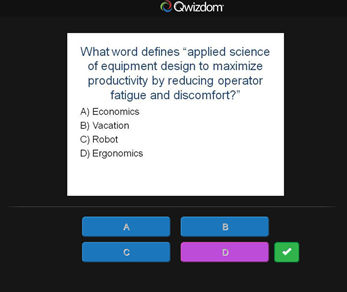
\includegraphics[]{qwizdom.png}
    \caption{Qwizdom web view for the audience}
    \label{fig:qwizdom}
\end{figure}

\section{Analysis}
% Taking into account the problem and what you learned from the background work,
% what was your analysis of the problem? How did your analysis help to decompose
% the problem into the main tasks that you would undertake? Were there alternative
% approaches? Why did you choose one approach compared to the alternatives?
%
% There should be a clear statement of the objectives of the work, which you will
% evaluate at the end of the work.
%
% In most cases, the agreed objectives or requirements will be the result of a compromise
% between what would ideally have been produced and what was determined to be possible in
%  the time available. A discussion of the process of arriving at the final list is usually appropriate.
%
% As mentioned in the lectures, think about possible security issues for the project topic.
%  Whilst these might not be relevant for all projects, do consider if there are relevant
%   for your project. Where there are relevant security issues, discuss how they will
%   this affect the work that you are doing. Carry forward this discussion into relevant
%    areas for design, implementation and testing.

% - MEAN stack \& Docker \& docker-compose
% - Version Control
% - build - Circle CI -> testing, autodeploy
% - AWS Production environment (did not know of Elasticbeanstalk at this point)
% - Google Single Sign On -> Security
% - Identification of major problems
% - Top level requirements of the system
\subsection{MEAN Stack}
Having considered various methods of developing the Quiz Tool, I have decided to
choose the web application approach, specifically to develop the application entirely
in JavaScript based technologies using the MEAN stack\cite{18}.
Allowing students to access the tool using both
their mobile devices and laptops, combined with the relatively low learning curve
both for me, and for anyone maintaining the software in the future, made it the best
option in my opinion.

MEAN stack consists of four elements:
\begin{itemize}
  \item \textbf{M}ongoDB is a JSON document storage NoSQL database
  \item \textbf{E}xpress is a minimalistic JavaScript web development framework
  \item \textbf{A}ngular is a front end web development framework
  \item \textbf{N}odeJS is a JavaScript engine
\end{itemize}

Front ends for both lecturers and students would be written in Angular, NodeJS would be
used on the back end together with Express, and the persistence layer would be provided
by MongoDB.

\subsection{Docker}
Each part of the application would be containerised using Docker\cite{19}, and containers
would run together in the same fashion on the developer's machine, and the build engine
using docker-compose\cite{20} container orchestration tool. Docker is an open source
engine which can be used to wrap an application and all its dependencies into a
lightweight container that can run on any machine capable of running containers\cite{21}.
Docker-compose on the other hand, is a tool for defining and running multi-container
Docker applications. Using Docker would make the development and testing of the Quiz
Tool easier, as any machine capable of running Docker containers, could run the tool.
It would also allow to easily change the production environment provider if necessary,
making it easier to maintain in the future.

\subsection{AWS Production Environment}
Unfortunately, the on-site hosting provided by the university to students to deploy
their final projects to was inadequate for the DevOps infrastructure I wanted to
put in place. I wanted to have a machine capable of running docker-compose, and some
form of continuous integration agent. The LXC debian containers\cite{22} were not
compatible with either docker-compose, or Jenkins\cite{23}. The Quiz Tool would be therefore
deployed to the production environment provided by an external cloud provider AWS\cite{24},
and an alternative build agent would be used. The GitHub Student Developer Pack\cite{25} offers
\$150 worth of credits for the Amazon cloud, which is why AWS was chosen.

\subsection{Build}
Continuous integration and deployment would be provided by Circle CI\cite{26}, as it is relatively easy
to work with and is very similar to Travis\cite{27}, while not being overly complex like Jenkins\cite{23}.
Its major advantage over its competitors is the ability to build projects stored in private
repositories, free of charge to a certain amount of build hours per month. Continuous integration
and deployment are software development industry practices that enable teams to reliably release
new features and products. Code is integrated and merged frequently, which shortens the release cycle,
improves code quality and team's productivity\cite{28}.

Build of the Quiz Tool should at the very least:
\begin{itemize}
  \item Checkout the source code from the version control
  \item Run all the tests
  \item Deploy the tool to the production environment when a production build runs
\end{itemize}

\subsection{Authentication and Security}
LDAP authentication could not be used with the production environment provided by
AWS. The alternative would be to use the Google Single Sign On\cite{2}, where lecturers
could login to the tool using their Google credentials. The major drawback of this
approach is that anyone with a Google account can login into the tool as a lecturer.
The major advantage is, that the credentials handling would be outsourced to Google,
making the Quiz Tool more secure and the tool would not have to store hashed passwords
by simply relying on the confirmation of user's identity by Google.

Having said that, Google ids would still be stored in MongoDB to uniquely identify
lecturers in the future, and to know who is the owner of lectures in the system.
Due to the fact that the interaction of the Docker containers making up the Quiz Tool would
be managed by docker-compose, the MongoDB container could be hidden from the outside world
and could be only accessed from the server container running the back end code. This would
make the database more secure.

Facebook and Twitter Single Sign On strategies\cite{facebook}\cite{twitter} were also
considered, however even though most people have a Facebook account, it is unlikely they
would like to use it to sign into a work related system. Twitter on the other hand,
was immediately rejected, as it is less common for people to use this platform.

\subsection{Top Level Requirements}
\label{subsection:toplevel}
Even though the tool would be developed using an agile approach, as described in the next
section of this document, certain top level functional requirements have been identified
before the development work had started. The initial conversation with the client (the
supervisor of the project) yielded the following requirements:

\begin{itemize}
  \item \textbf{FR-1} - Add a login page for lecturers. As a lecturer it should be possible to login
  into the tool using lecturer's credentials.
  \item \textbf{FR-2} - Add a login page for students. As a student it should be possible to join
  an ongoing session using the session code provided by the lecturer.
  \item \textbf{FR-3} - Add a dashboard for lecturers to upload their lecture slides to.
  \item \textbf{FR-4} - Add the ability to add quizzes to lectures.
  \item \textbf{FR-5} - Add the ability to broadcast lectures.
  \item \textbf{FR-6} - Add the ability to export lecture session results in some format
  for future analysis.
\end{itemize}

\section{Process}
\subsection{Version Control}
\label{subsection:versioncontrol}
Git\cite{29} would be used for the version control during the development of the Quiz Tool, together with
the GitHub\cite{30} web-based hosting service. The source code would be stored in a private
repository. There would be a \texttt{master} production branch, and suitable guards would be added
so that new code cannot be pushed directly to the production branch. The feature-branch git
workflow\cite{31} would be used and each \texttt{feature-branch} would need to have an associated issue
(story) on GitHub. Then a pull request could be opened between the \texttt{feature-branch} and the \texttt{master}
branch, and Circle CI would checkout the code, run all tests and report back to GitHub to either
allow the merge or block it, depending on whether the build was successful or not. Once the pull request
is merged into \texttt{master}, a production build would run, where Circle CI would checkout the code, run
all the tests and finally automatically deploy the new version of the Quiz Tool to the production
environment provided by AWS.

A Kanban board provided by the ZenHub Chrome plugin\cite{32} would be used. It would allow issues to be grouped
into epics, and each story could have a corresponding amount of points assigned to it, depending
on the likely complexity of the task. For example a single point would correspond to half day of work.

\subsection{Development Methodology}
\label{subsection:scrum}
The application would be developed using the SCRUM methodology adjusted for a single person project.
An agile approach was chosen, as even though the top level requirements were known, it would
be very difficult to plan the entire system ahead, before developing it by following a traditional,
waterfall methodology. Evolutionary design would also allow for quick changes if the tool
did not meet client's expectations half way through the development. Certain elements of the full
SCRUM would be used as described below, however daily scrums would be removed, as there would
be no point of having a single person stand up by myself.

The development work would be split into weekly sprints. Each sprint would start with sprint
planning, where issues would be created and their complexity would be estimated using ZenHub
story points. During the week, issues would be tackled, and the progress could be monitored using
the Kanban board. GitHub labels would be used to quickly differentiate between different types
of issues. For example there would be a different coloured label for front end tasks, back end
tasks, documentation, DevOps etc. Time commitment would also be tracked on day to day basis
using a Google Sheets spreadsheet\cite{33}. Each sprint would end with a sprint retrospective, where
a document would be produced containing a list of things that went well during the week, and things
that could be improved. Weekly meetings with the client (supervisor) would provide immediate feedback
on work done and allow re-adjustment of the approach necessary to stay on track to deliver the
software before the deadline. Finally, velocity would be tracked and burn down charts automatically
produced following each iteration. This would give more confidence in estimating the future work.


% You need to describe briefly the life cycle model or research method that you used. You
%  do not need to write about all of the different process models that you are aware of.
%  Focus on the process model that you have used. It is possible that you needed to adapt
%  an existing process model to suit your project; clearly identify what you used and how
%  you adapted it for your needs.
